\chapter{Phase 3 - Mit Änderungen der Hardware}
\label{ch:phase3}
War die Infrastruktur von WLAN Access Points bisher gegeben und die Hardware somit unveränderlich, soll diese nun ausstauschbar beziehungsweise erweiterbar sein.
Dies erlaubt die Implementierung eines Bereichsortungssystems, welches nicht an die 802.11 Spezifikation gebunden ist.
Es soll eine Funkübetragungstechnik gewählt werden, die es den Tags erlaubt die in Abschnitt \ref{ch:Einleitung:sec:Anforderungen} maximal geforderten 3 Jahre Akkulaufzeit zu erreichen.
Da mehrere Topologien für das Knotennetzwerk denkbar sind, werden die Begriffe Knoten und AP im Folgenden nicht mehr gleichgesetzt.
Eine Möglichkeit wäre, APs einzusetzen, die eine zweite Funkübetragungstechnik beherrschen, optional könnnte diese Fähigkeit etwa über einen USB-Port nachgerüstet werden.
Stattdessen kann die neu eingesetzte Technik auch von der bestehenden Infrastruktur getrennt und eine neue Infrastruktur aus Knoten aufgebaut werden.
Als Kompromiss der vorherigen Möglichkeiten können sich die neuen Knoten auch mittels LAN oder WLAN in die bestehende Infrastruktur einfügen. 
Dieser Kompromiss ist grundsätzlich zu bevorzugen, da er die Komplexität geringer als bei zwei eigenständigen Netzen ist.

\section{Vorherige Arbeiten}
\label{ch:phase3:sec:vorherige}


\subsection{Geeignete Messwerte für Bluetooth}
Hossain et al. untersuchen die laut Bluetooth Spezifikation zurückgegebenen Messwerte bezüglich ihrer Eignung für die Lokalisierung \cite{hossain2007comprehensive}.\\ 
Link Quality (LQ) beschreibt, wie gut die Verbindung zwischen zwei Geräten ist.
Der Wert wird aus der Bitfehlerrate beim Empfänger berechnet, allerdings ist nicht spezifiziert, wie der Wert zu berechnen ist, er hängt also in hohem Maße vom Hersteller des Empfängers ab. \\
Der Received Signal Strength Indicator (RSSI) misst die Stärke des eingehenden Signals, die Spezifikation sieht jedoch eine Golden Receive Power Range (GRPR) vor. 
Liegt der RSSI über oder unter dieser wird eine Anfrage zum erhöhen oder verringern der Sendeleistung an das andere Gerät verschickt, dies dient während einer aktiven Verbindung dazu den Energieverbrauch zu senken.
Problematisch am RSSI ist, dass er relativ zur GRPR bestimmt wird.
In der Untersuchung von Hossain et al. führte das dazu, dass der RSSI mit 0 gemessen wurde, wenn er innerhalb der GRPR lag. \\
Transmission Power Level (TPL) ist die Sendeleistung eines Geräts. 
TPL kann während einer bestehenden Verbindung durch Anfragen des Verbindungspartners verändert werden.
Dazu muss diese Energiesparfunktion jedoch unterstützt werden, was bei dem von Hossain et al. vwrwendeten Gerät nicht der Fall war.
Abb. \ref{fig:bluetoothmess} zeigt deshalb für TPL eine waagerechte Linie.\\
Für Inquirys wird die Stärke des eingehenden Signals ohne die Beactung des GRPR bestimmt.
Außerdem werden Inquirys immer mit voller Sendeleistung gesendet, da sie zur Entdeckung von Ressourcen verwendet werden.
Es handelt sich ebenfalls um den RSSI, um jedoch den Unterschied zum RSSI für eine Verbindung deutlich zu machen nennen Hossain et al. diesen Wert RX Power Level.

\begin{figure}[h]
  \centering
	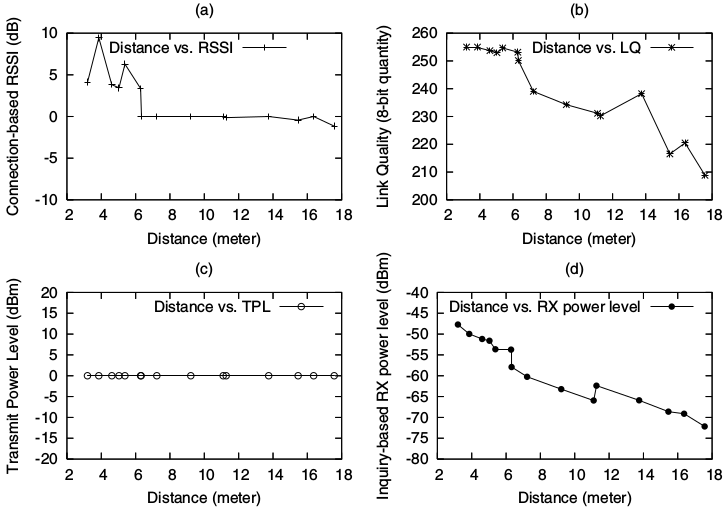
\includegraphics[width=\textwidth]{images/bluetoothmess.png}
  \caption{Korrelation der Messwerte mit der Distanz, aus \cite{hossain2007comprehensive}}
  \label{fig:bluetoothmess}
\end{figure}

\subsection{RSSI-basierte BLE Ortung}
Jianyong et al. stellen ein System zur Ortung auf Basis von Bluetooth Low Energie (BLE, auch Bluetooth Smart) vor \cite{jianyong2014rssi}. \\
Sie messen an den Knoten den RSSI von Inquiry Paketen die zuvor von den mobilen Einheiten versendet wurden.
Für die genaue Ortung werden die Ergebnisse mit einem Gauß-Filter geglättet und für jeden Knoten die Parameter für ein Signalausbreitungsmodell bestimmt.
Das gemessene Signalstärke $P = A - 10n*log(d)$ hängt von der Referenzsignalstärke A im Abstand von einem Meter, dem Dämpfungsfaktor n und der Distanz d ab. \\
Jianyong et al. bestimmen die Referenzsignalstärke und den Dämpfungsfaktor für jeden Knoten.
Da jedoch nur eine Bereichsortung für diese Arbeit gefordert wurde, sollten A und n nur beispielhaft für einen Knoten bestimmt werden, um den Aufwand beim Aufbau der Infrastruktur zu reduzieren.
Abb. \ref{fig:blemodel} zeigt die von Jianyong et al. bestimmten Parameter für das Signalausbreitungsmodell. 
Abb. \ref{fig:blemodel} zeigt außerdem, dass die verwendeten CC2540 Development Kit von Texas Instruments von einem Access Point nur auf 20 Meter detektiert werden konnte.

\begin{figure}[h]
  \centering
	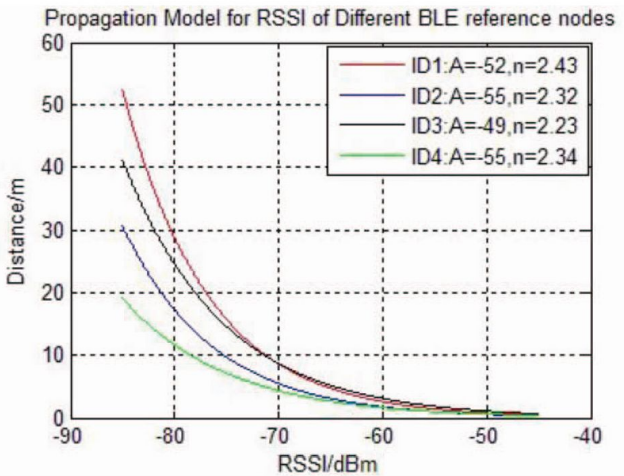
\includegraphics[width=0.7\textwidth]{images/blemodel.png}
  \caption{Signalausbreitungsmodelle aus \cite{jianyong2014rssi}}
  \label{fig:blemodel}
\end{figure}
